\documentclass{article}\usepackage[]{graphicx}\usepackage[]{color}
%% maxwidth is the original width if it is less than linewidth
%% otherwise use linewidth (to make sure the graphics do not exceed the margin)
\makeatletter
\def\maxwidth{ %
  \ifdim\Gin@nat@width>\linewidth
    \linewidth
  \else
    \Gin@nat@width
  \fi
}
\makeatother

\definecolor{fgcolor}{rgb}{0.345, 0.345, 0.345}
\newcommand{\hlnum}[1]{\textcolor[rgb]{0.686,0.059,0.569}{#1}}%
\newcommand{\hlstr}[1]{\textcolor[rgb]{0.192,0.494,0.8}{#1}}%
\newcommand{\hlcom}[1]{\textcolor[rgb]{0.678,0.584,0.686}{\textit{#1}}}%
\newcommand{\hlopt}[1]{\textcolor[rgb]{0,0,0}{#1}}%
\newcommand{\hlstd}[1]{\textcolor[rgb]{0.345,0.345,0.345}{#1}}%
\newcommand{\hlkwa}[1]{\textcolor[rgb]{0.161,0.373,0.58}{\textbf{#1}}}%
\newcommand{\hlkwb}[1]{\textcolor[rgb]{0.69,0.353,0.396}{#1}}%
\newcommand{\hlkwc}[1]{\textcolor[rgb]{0.333,0.667,0.333}{#1}}%
\newcommand{\hlkwd}[1]{\textcolor[rgb]{0.737,0.353,0.396}{\textbf{#1}}}%

\usepackage{framed}
\makeatletter
\newenvironment{kframe}{%
 \def\at@end@of@kframe{}%
 \ifinner\ifhmode%
  \def\at@end@of@kframe{\end{minipage}}%
  \begin{minipage}{\columnwidth}%
 \fi\fi%
 \def\FrameCommand##1{\hskip\@totalleftmargin \hskip-\fboxsep
 \colorbox{shadecolor}{##1}\hskip-\fboxsep
     % There is no \\@totalrightmargin, so:
     \hskip-\linewidth \hskip-\@totalleftmargin \hskip\columnwidth}%
 \MakeFramed {\advance\hsize-\width
   \@totalleftmargin\z@ \linewidth\hsize
   \@setminipage}}%
 {\par\unskip\endMakeFramed%
 \at@end@of@kframe}
\makeatother

\definecolor{shadecolor}{rgb}{.97, .97, .97}
\definecolor{messagecolor}{rgb}{0, 0, 0}
\definecolor{warningcolor}{rgb}{1, 0, 1}
\definecolor{errorcolor}{rgb}{1, 0, 0}
\newenvironment{knitrout}{}{} % an empty environment to be redefined in TeX

\usepackage{alltt}
\usepackage[utf8]{inputenc}
\usepackage{amsmath}
\usepackage{graphicx}
%\usepackage{bbold}
\usepackage{tikz}
%\usepackage{silence}
\usepackage{mdframed}
%\WarningFilter{mdframed}{You got a bad break}
\usepackage[colorinlistoftodos]{todonotes}
\usepackage{listings}
\usepackage{color}
\colorlet{exampcol}{blue!10}
\usepackage{multicol}
\usepackage{booktabs}

\title{BIO311: Population Ecology\\ \textit{Practical 6: An introduction to \texttt{R}}}
\setlength\parindent{0pt}

\setcounter{tocdepth}{1} % Determines the depth of the table of contents;; 0:chapters, 1: chapters and sections, 2: chapters,sections and subsections

%\renewcommand{\theExercise}{\thechapter.\arabic{Exercise}}%
\IfFileExists{upquote.sty}{\usepackage{upquote}}{}
\begin{document}

\author{Timoth\'ee Bonnet \&\footnote{This document was co-authored by Tina Cornioley}\; Koen van Benthem\\\\
\tt{timothee.bonnet@ieu.uzh.ch}\\ \tt{koen.vanbenthem@ieu.uzh.ch}}

\date{Spring 2016}




\maketitle
\tableofcontents
\vspace{3cm}
\begin{mdframed}
\textit{We do not claim to teach you the most efficient way to use \texttt{R}. If you at some point during the computer practicals encounter a code that you could make more efficient or elegant, please do let us know! We do want to learn from you as well.\\[1.5ex] However, do try to understand exactly what we are doing and how the functions we use work. The best way to learn how functions work is by either using the \texttt{R}-manaul (type \texttt{?functionname}) or by creating dummy data (just make up a small amount of data yourself) and analyse what the function does to this data.}
\end{mdframed}
\newpage
\section{Getting to know \texttt{R}}
Before exploring the data that you collected in the lab, we recommend you to get familiar with \texttt{R}. Please go over the following tutorial up to and including section 6 to learn or refresh the basics of \texttt{R}:\\

\texttt{http://cran.r-project.org/doc/contrib/Torfs+Brauer-Short-R-Intro.pdf}
\vspace{1.5ex}

\textit{Note: in this tutorial the word vector is used for all lists of numbers and the word matrix is used for all arrays of numbers, not only for transformations.}

\begin{mdframed}[backgroundcolor=red!40]
\textbf{In this document you will find both normal text as well as \texttt{R}-code. Copying code from this pdf into \texttt{R} may results in errors. This has to do with the encoding of the file. Instead we recommend to retype the commands.}
\end{mdframed}

\section{Dataset preparation}
Prepare you dataset in excel before importing it into \texttt{R}. Open your rotifer data in excel and create a copy. Never directly modify your original data file. There is always the chance that you make a serious mistake which results in losing all or part of your data. Your file must not contain any space (especially check the column names, they should have no space between words) or any special character of the type "\'e" or "\"o". Remove the comments, they are not in a form that can be analysed numerically but keep them in mind when writing your report. Avoid empty cells by filling them with \texttt{NA} if you do not know the value for that cell or zero if appropriate. 


Once you have checked your document, save it as a .csv file delimited with ",". Carefully select the folder you save your document into. You will have to set this folder as your working directory later. If you are new to \texttt{R}, the easiest is that you save it in a folder name "Pop\textunderscore Ecol" on your desktop.

\section{Getting data into \texttt{R}}
\subsection{Step 1: Set the working directory}
This is the folder where \texttt{R} will search for files and where it will save your data afterwards. You must insert your own working directory path.

Making a mistake when typing the directory path from memory is very likely. Instead, you can right-click your file and select "Properties". From here, you can copy and paste the full directory structure (and the file name). 
\begin{knitrout}
\definecolor{shadecolor}{rgb}{0.969, 0.969, 0.969}\color{fgcolor}\begin{kframe}
\begin{alltt}
\hlkwd{setwd}\hlstd{(}\hlstr{"C:/Desktop/Pop_Ecol"}\hlstd{)}
\end{alltt}
\end{kframe}
\end{knitrout}
\subsection{Step 2: Load your dataset}
The next step is loading your dataset into \texttt{R}. The line of code below shows how to read your dataset if it is saved as \texttt{'rotifer\textunderscore data.csv'} file seperated with ",". The dataset must be in the working directory you specified above otherwise this command won't work.
\begin{knitrout}
\definecolor{shadecolor}{rgb}{0.969, 0.969, 0.969}\color{fgcolor}\begin{kframe}
\begin{alltt}
\hlstd{rot}\hlkwb{<-}\hlkwd{read.csv}\hlstd{(}\hlstr{"rotifer_data.csv"}\hlstd{,} \hlkwc{sep}\hlstd{=}\hlstr{","}\hlstd{,} \hlkwc{header}\hlstd{=T)}
\end{alltt}
\end{kframe}
\end{knitrout}
\subsection{Step 3: Check your data}
\subsubsection{Initial overview}
The next functions allow you to take a first look at the data you have loaded. If you see anything strange at this stage, you may have to go back to your original document in excel.
\begin{knitrout}
\definecolor{shadecolor}{rgb}{0.969, 0.969, 0.969}\color{fgcolor}\begin{kframe}
\begin{alltt}
\hlkwd{head}\hlstd{(rot)} \hlcom{# Output the first few rows of rot}
\hlkwd{tail}\hlstd{(rot)} \hlcom{# Output the last few rows of rot}
\hlkwd{str}\hlstd{(rot)}  \hlcom{# Describe the structure of rot}
\hlkwd{summary}\hlstd{(rot)} \hlcom{# Calculate basic information for each column in rot}
\end{alltt}
\end{kframe}
\end{knitrout}
What happens if you type \texttt{head(rot,10)} instead of \texttt{head(rot)}? Try the same thing for the function \texttt{tail}.
\subsubsection{Finding typos}
While typing in the data, a typo is easily made, especially for the columns \texttt{Copper} and \texttt{Population}. For the rest of the analysis it is crucial that the spelling in these columns is consistent. For this, we focus on these specific columns. To access one specific column, we use the notation \texttt{dataframe\$columnname}. Thus, to extract all the values of the \texttt{Population} column, you can use \texttt{rot\$Population}. Now use the command \texttt{table()} to obtain a summary of this data:
\begin{knitrout}
\definecolor{shadecolor}{rgb}{0.969, 0.969, 0.969}\color{fgcolor}\begin{kframe}
\begin{alltt}
\hlkwd{table}\hlstd{(rot}\hlopt{$}\hlstd{Population)}
\end{alltt}
\end{kframe}
\end{knitrout}
You will notice that the post pollution populations are indicated with either \texttt{Postpollution} or \texttt{Post-pollution}. This will be very inconvenient in the further analysis. Correct this as follows:
\begin{knitrout}
\definecolor{shadecolor}{rgb}{0.969, 0.969, 0.969}\color{fgcolor}\begin{kframe}
\begin{alltt}
\hlstd{rot}\hlopt{$}\hlstd{Population[rot}\hlopt{$}\hlstd{Population}\hlopt{==}\hlstr{"Post-pollution"}\hlstd{]}\hlkwb{<-}\hlstr{"Postpollution"}
\end{alltt}
\end{kframe}
\end{knitrout}
What happens here is that we first select the column \texttt{Population} by typing \texttt{rot\$Population}. Next, the square brackets indicate that we are only interested in a part of the contents of that column. The part that we are interested in, are the entries that have the value \texttt{"Post-pollution"}. Precisely these elements are selected by \texttt{rot\$Population[rot\$Population=="Post-pollution"]}. Subsequently these elements are replaced by the properly spelled version by the command \texttt{<-"Postpollution"}. Now we check whether the problem is solved:
\begin{knitrout}
\definecolor{shadecolor}{rgb}{0.969, 0.969, 0.969}\color{fgcolor}\begin{kframe}
\begin{alltt}
\hlkwd{table}\hlstd{(rot}\hlopt{$}\hlstd{Population)}
\end{alltt}
\begin{verbatim}
## 
##    Commercial     Pollution Postpollution      Recovery 
##            54            54            54            54
\end{verbatim}
\end{kframe}
\end{knitrout}
Repeat these steps now for the \texttt{Copper} column, and correct any typos you encounter in that column.
\begin{mdframed}
\textit{Please note that we have included these errors manually, just for practicing purposes.}
\end{mdframed}

\subsubsection{Average values per type}
So far we have looked at a set of summary statistics for the \texttt{rot} dataframe. These statistics were however all calculated for the full dataset, regardless of the parameters. In reality we would like to show such statistics per type (that is unique combination of \texttt{Population}, \texttt{Copper} and \texttt{Day}). Below we use the \texttt{aggregate()} function to calculate the mean number of alive juveniles for unique combinations of \texttt{Copper} and \texttt{Population}. Please extend this code to also account for the different days.
\begin{knitrout}
\definecolor{shadecolor}{rgb}{0.969, 0.969, 0.969}\color{fgcolor}\begin{kframe}
\begin{alltt}
\hlkwd{aggregate}\hlstd{(rot}\hlopt{$}\hlstd{Alive_Juv,}\hlkwc{by}\hlstd{=}\hlkwd{list}\hlstd{(rot}\hlopt{$}\hlstd{Population,rot}\hlopt{$}\hlstd{Copper),mean)}
\end{alltt}
\begin{verbatim}
##          Group.1 Group.2        x
## 1     Commercial    high 5.888889
## 2      Pollution    high 2.055556
## 3  Postpollution    high 1.722222
## 4       Recovery    high 2.611111
## 5     Commercial     low 7.111111
## 6      Pollution     low 2.666667
## 7  Postpollution     low 1.666667
## 8       Recovery     low 2.944444
## 9     Commercial  medium 5.833333
## 10     Pollution  medium 3.833333
## 11 Postpollution  medium 2.444444
## 12      Recovery  medium 1.888889
\end{verbatim}
\end{kframe}
\end{knitrout}
Now repeat this procedure to also calculate the average number of alive adults per \texttt{Population}, \texttt{Copper}-treatment and \texttt{Day}.

Finally adapt the script to also calculate other parameters, such as the median, maximum counts, minimum counts, standard deviation and variance.

\subsection{Step 4: Plot your data}
Let us have a look at how your rotifer population does over time. For this we use the \texttt{plot} function in \texttt{R}. The first argument contains the \texttt{x} variables and the second the \texttt{y} variables.
\begin{knitrout}
\definecolor{shadecolor}{rgb}{0.969, 0.969, 0.969}\color{fgcolor}

{\centering \includegraphics[width=0.5\textwidth]{figure/aagp5-1} 

}



\end{knitrout}
However, if we call the function like this, \texttt{R} wil automatically set the axis (the limits and the location of the tick marks). This is okay for quick plots, but for reports you will probably want a bit more control. One way to do so is shown in the following.

We will focus first on the populations with the low copper treatment. For simplicity we will only look at the total population numbers. Start by making an empty plot with the correct labels then draw the axes in this plot. Later we will lines add lines to this plot:
\begin{knitrout}
\definecolor{shadecolor}{rgb}{0.969, 0.969, 0.969}\color{fgcolor}\begin{kframe}
\begin{alltt}
\hlkwd{plot}\hlstd{(}\hlnum{0}\hlstd{,}\hlnum{0}\hlstd{,}\hlkwc{type}\hlstd{=}\hlstr{"n"}\hlstd{,}\hlkwc{xlab}\hlstd{=}\hlstr{"Day"}\hlstd{,}
     \hlkwc{ylab}\hlstd{=}\hlstr{"Total population size"}\hlstd{,}
     \hlkwc{main}\hlstd{=}\hlstr{"Low copper treatment"}\hlstd{,}
     \hlkwc{axes}\hlstd{=}\hlnum{FALSE}\hlstd{,}\hlkwc{xlim}\hlstd{=}\hlkwd{c}\hlstd{(}\hlnum{1}\hlstd{,}\hlnum{3}\hlstd{),}\hlkwc{ylim}\hlstd{=}\hlkwd{c}\hlstd{(}\hlnum{0}\hlstd{,}\hlnum{30}\hlstd{))}
\hlkwd{axis}\hlstd{(}\hlkwc{side}\hlstd{=}\hlnum{1}\hlstd{,}\hlkwc{at}\hlstd{=}\hlkwd{c}\hlstd{(}\hlnum{1}\hlstd{,}\hlnum{2}\hlstd{,}\hlnum{3}\hlstd{))}
\hlkwd{axis}\hlstd{(}\hlkwc{side}\hlstd{=}\hlnum{2}\hlstd{,} \hlkwc{at}\hlstd{=}\hlkwd{c}\hlstd{(}\hlnum{0}\hlstd{,}\hlnum{5}\hlstd{,}\hlnum{10}\hlstd{,}\hlnum{15}\hlstd{,}\hlnum{20}\hlstd{,}\hlnum{25}\hlstd{,}\hlnum{30}\hlstd{))}
\end{alltt}
\end{kframe}
\end{knitrout}
Now we need to prepare the data that we are interested in. First we use the \texttt{factor()} function in the beginning to make sure that the variable \texttt{Population} will be plot in the correct order. Furthermore we add a new variable \texttt{Total} that corresponds to the total number of individuals (adults and juveniles).
\begin{knitrout}
\definecolor{shadecolor}{rgb}{0.969, 0.969, 0.969}\color{fgcolor}\begin{kframe}
\begin{alltt}
\hlstd{rot}\hlopt{$}\hlstd{Population}\hlkwb{=}\hlkwd{factor}\hlstd{(rot}\hlopt{$}\hlstd{Population,}
                      \hlkwc{levels}\hlstd{=}\hlkwd{c}\hlstd{(}\hlstr{'Commercial'}\hlstd{,}\hlstr{'Postpollution'}\hlstd{,}
                        \hlstr{'Recovery'}\hlstd{,}\hlstr{'Pollution'}\hlstd{),} \hlkwc{ordered}\hlstd{=T)}

\hlstd{rot}\hlopt{$}\hlstd{Total} \hlkwb{<-} \hlstd{rot}\hlopt{$}\hlstd{Alive_Juv} \hlopt{+} \hlstd{rot}\hlopt{$}\hlstd{Alive_Adult}
\end{alltt}
\end{kframe}
\end{knitrout}
To select only the low copper treatment entries, use the function \texttt{subset()} and store this part of the dataset in a new variable \texttt{temp}. Make sure you understand what this function does.
\begin{knitrout}
\definecolor{shadecolor}{rgb}{0.969, 0.969, 0.969}\color{fgcolor}\begin{kframe}
\begin{alltt}
\hlstd{temp}\hlkwb{<-}\hlkwd{subset}\hlstd{(rot,Copper}\hlopt{==}\hlstr{'low'}\hlstd{)}
\end{alltt}
\end{kframe}
\end{knitrout}
Next use \texttt{aggregate()} to calculate the mean number of total individuals alive per day and population. Store this information in a variable named \texttt{Tot\textunderscore mean}. This should give you:
\begin{center}
% latex table generated in R 3.2.2 by xtable 1.7-4 package
% Tue Mar  8 18:38:49 2016
{\footnotesize
\begin{tabular}{lrr}
 Group.1 & Group.2 & x \\ 
  \hline
Commercial &   1 & 6.00 \\ 
  Postpollution &   1 & 6.00 \\ 
  Recovery &   1 & 6.00 \\ 
  Pollution &   1 & 6.00 \\ 
  Commercial &   2 & 11.17 \\ 
  Postpollution &   2 & 3.00 \\ 
  Recovery &   2 & 6.33 \\ 
  Pollution &   2 & 6.50 \\ 
  Commercial &   3 & 23.00 \\ 
  Postpollution &   3 & 4.50 \\ 
  Recovery &   3 & 8.33 \\ 
  Pollution &   3 & 10.67 \\ 
  \end{tabular}
}

\end{center}
Now we use the command \texttt{lines()} to add a line for the commercial populations to the empty plot:
\begin{knitrout}
\definecolor{shadecolor}{rgb}{0.969, 0.969, 0.969}\color{fgcolor}\begin{kframe}
\begin{alltt}
\hlstd{temp2}\hlkwb{<-}\hlkwd{subset}\hlstd{(Tot_mean,Group.1}\hlopt{==}\hlstr{"Commercial"}\hlstd{)}
\hlkwd{lines}\hlstd{(temp2}\hlopt{$}\hlstd{Group.2,temp2}\hlopt{$}\hlstd{x,}\hlkwc{col}\hlstd{=}\hlstr{'red'}\hlstd{,}\hlkwc{pch}\hlstd{=}\hlnum{1}\hlstd{,}\hlkwc{type}\hlstd{=}\hlstr{"b"}\hlstd{)}
\end{alltt}
\end{kframe}

{\centering \includegraphics[width=0.5\textwidth]{figure/gp5-1} 

}



\end{knitrout}
Use these methods to also add lines for the other populations.\\
\begin{knitrout}
\definecolor{shadecolor}{rgb}{0.969, 0.969, 0.969}\color{fgcolor}

{\centering \includegraphics[width=0.5\textwidth]{figure/gp6-1} 

}



\end{knitrout}
We are getting closer, but we aren't there yet, now we want to add a legend to the figure. To do so we use the command \texttt{legend()}, with $7$ parameters. Use \texttt{?legend} to find out what each parameter determines (or just play around with the parameters to find that out):
\begin{knitrout}
\definecolor{shadecolor}{rgb}{0.969, 0.969, 0.969}\color{fgcolor}\begin{kframe}
\begin{alltt}
\hlkwd{legend}\hlstd{(}\hlkwc{x}\hlstd{=}\hlnum{1}\hlstd{,} \hlkwc{y}\hlstd{=}\hlnum{24}\hlstd{,} \hlkwc{col}\hlstd{=}\hlkwd{c}\hlstd{(}\hlstr{"red"}\hlstd{,}\hlstr{"blue"}\hlstd{,}\hlstr{"green"}\hlstd{,}\hlstr{"orange"}\hlstd{),}
\hlkwc{legend}\hlstd{=}\hlkwd{c}\hlstd{(}\hlstr{"Commercial"}\hlstd{,}\hlstr{"Postpollution"}\hlstd{,}\hlstr{"Recovery"}\hlstd{,}\hlstr{"Pollution"}\hlstd{),}
\hlkwc{lty}\hlstd{=}\hlnum{1}\hlstd{,} \hlkwc{pch}\hlstd{=}\hlnum{1}\hlstd{,} \hlkwc{bty}\hlstd{=}\hlstr{"n"}\hlstd{)}
\end{alltt}
\end{kframe}

{\centering \includegraphics[width=0.5\textwidth]{figure/gp7-1} 

}



\end{knitrout}
Finally we would like to introduce error bars in this graph. To do so, we first define a function for calculating the standard error. The standard error ($SE$) is defined as the standard deviation ($sd$) divided by the square root of the number of measurements ($N$) that the mean depends on:
\begin{equation*}
SE = \frac{\sigma}{\sqrt{N}}.
\end{equation*}
We use this property to define a new function that calculates the standard error:
\begin{knitrout}
\definecolor{shadecolor}{rgb}{0.969, 0.969, 0.969}\color{fgcolor}\begin{kframe}
\begin{alltt}
\hlstd{SE}\hlkwb{<-}\hlkwa{function}\hlstd{(}\hlkwc{x}\hlstd{)} \hlkwd{sd}\hlstd{(x)}\hlopt{/}\hlkwd{sqrt}\hlstd{(}\hlkwd{length}\hlstd{(x))}
\end{alltt}
\end{kframe}
\end{knitrout}
If we now call \texttt{SE(x)}, it will return us the standard error of \texttt{x}. We use this function together with \texttt{aggregate} to calculate the standard errors for all our datapoints in the low copper treatment:
\begin{center}
\begin{kframe}
\begin{alltt}
\hlstd{SE_tot}\hlkwb{<-}\hlkwd{aggregate}\hlstd{(temp}\hlopt{$}\hlstd{Total,}\hlkwc{by}\hlstd{=}\hlkwd{list}\hlstd{(temp}\hlopt{$}\hlstd{Population,temp}\hlopt{$}\hlstd{Day),SE)}
\end{alltt}
\end{kframe}% latex table generated in R 3.2.2 by xtable 1.7-4 package
% Tue Mar  8 18:38:51 2016
{\footnotesize
\begin{tabular}{lrr}
 Group.1 & Group.2 & x \\ 
  \hline
Commercial &   1 & 0.00 \\ 
  Postpollution &   1 & 0.00 \\ 
  Recovery &   1 & 0.00 \\ 
  Pollution &   1 & 0.00 \\ 
  Commercial &   2 & 0.95 \\ 
  Postpollution &   2 & 1.06 \\ 
  Recovery &   2 & 0.49 \\ 
  Pollution &   2 & 1.20 \\ 
  Commercial &   3 & 2.62 \\ 
  Postpollution &   3 & 1.54 \\ 
  Recovery &   3 & 1.12 \\ 
  Pollution &   3 & 2.14 \\ 
  \end{tabular}
}

\end{center}
Finally we use the function \texttt{arrows()} (use \texttt{?arrows} to understand how this function works or play around with the parameters to see the effects) to add the error bars. For the commercial populations this would work as follows:
\begin{knitrout}
\definecolor{shadecolor}{rgb}{0.969, 0.969, 0.969}\color{fgcolor}\begin{kframe}
\begin{alltt}
\hlstd{temp2}\hlkwb{<-}\hlkwd{subset}\hlstd{(Tot_mean,Group.1}\hlopt{==}\hlstr{"Commercial"}\hlstd{)}
\hlstd{temp3}\hlkwb{<-}\hlkwd{subset}\hlstd{(SE_tot,Group.1}\hlopt{==}\hlstr{"Commercial"}\hlstd{)}
\hlkwd{arrows}\hlstd{(temp3}\hlopt{$}\hlstd{Group.2,temp2}\hlopt{$}\hlstd{x}\hlopt{-}\hlstd{temp3}\hlopt{$}\hlstd{x,temp3}\hlopt{$}\hlstd{Group.2,temp2}\hlopt{$}\hlstd{x}\hlopt{+}\hlstd{temp3}\hlopt{$}\hlstd{x,}
       \hlkwc{angle}\hlstd{=}\hlnum{90}\hlstd{,}\hlkwc{length}\hlstd{=}\hlnum{0.1}\hlstd{,}\hlkwc{col}\hlstd{=}\hlstr{'red'}\hlstd{,}\hlkwc{code}\hlstd{=}\hlnum{3}\hlstd{)}
\end{alltt}
\end{kframe}
\includegraphics[width=\maxwidth]{figure/gp10-1} 

\end{knitrout}
You will notice a warning message about zero-length arrows. What does this mean? Repeat this procedure to also include error bars for the other three lines. Can you now also generate the plots for the other two copper treatments? 
\begin{knitrout}
\definecolor{shadecolor}{rgb}{0.969, 0.969, 0.969}\color{fgcolor}

{\centering \includegraphics[width=0.65\textwidth]{figure/gekkeplot-1} 

}




{\centering \includegraphics[width=0.65\textwidth]{figure/gekkeplot-2} 

}




{\centering \includegraphics[width=0.65\textwidth]{figure/gekkeplot-3} 

}



\end{knitrout}
\begin{mdframed}
\textit{The shortcut}\\
First of all the code can be shortened by using for-loops, can you find two place where introducing a for-loop would make the code shorter? Besides, we are not the first people to deal with this problem: actually the sciplot package does all of this in a more or less automated way:
\begin{knitrout}
\definecolor{shadecolor}{rgb}{0.969, 0.969, 0.969}\color{fgcolor}\begin{kframe}
\begin{alltt}
\hlkwd{library}\hlstd{(sciplot)}
\hlstd{temp}\hlkwb{<-}\hlkwd{subset}\hlstd{(rot,}\hlkwc{Copper}\hlstd{=}\hlstr{'low'}\hlstd{)}
\hlkwd{lineplot.CI}\hlstd{(temp}\hlopt{$}\hlstd{Day,temp}\hlopt{$}\hlstd{Total,}
            \hlkwc{group}\hlstd{=temp}\hlopt{$}\hlstd{Population,}\hlkwc{fixed}\hlstd{=T,} \hlkwc{ylim}\hlstd{=}\hlkwd{c}\hlstd{(}\hlnum{0}\hlstd{,}\hlnum{26}\hlstd{),}
            \hlkwc{xlab}\hlstd{=}\hlstr{"Day"}\hlstd{,}\hlkwc{ylab}\hlstd{=}\hlstr{"Total population size"}\hlstd{,}
            \hlkwc{main}\hlstd{=}\hlstr{"Low copper treatment"}\hlstd{)}
\end{alltt}
\end{kframe}

{\centering \includegraphics[width=0.6\textwidth]{figure/blabla-1} 

}



\end{knitrout}
\end{mdframed}
\subsection{Saving your graph}
If you want to save your graph, write the code in R following the instructions below:
\begin{enumerate}
\item Choose a file name. This can be anything, for example, ''Nameyourgraph.jpg''.
\item Open a jpeg file by typing jpeg(file = ''Nameyourgraph.jpg'').
\item Use the plot command to make graphs. Because you typed the jpeg command, R will send all graphs to the jpeg file, and the graphic output will not appear on the screen.
\item Close the jpeg file by typing: \texttt{dev.off()}.
\end{enumerate}
\begin{mdframed}
\textbf{File types for images}\\
In the example above we have described how to save a graph as a \texttt{jpg}. Saving your graph as a \texttt{jpg} is not always the best way to go. As you may notice the quality of the output is not always as good. You can try to increase the quality of the image by adding the parameters \texttt{width} and \texttt{height} to the \texttt{jpg} command. We will now compare two graphs, each with different numbers for the \texttt{width} and \texttt{height:}. We have cut out the axis labels for comparison purposes.

\begin{knitrout}
\definecolor{shadecolor}{rgb}{0.969, 0.969, 0.969}\color{fgcolor}\begin{kframe}
\begin{alltt}
\hlstd{x}\hlkwb{<-}\hlnum{1}\hlopt{:}\hlnum{5}
\hlstd{y}\hlkwb{<-}\hlkwd{runif}\hlstd{(}\hlnum{5}\hlstd{)}
\hlkwd{jpeg}\hlstd{(}\hlstr{'jpg1.jpg'}\hlstd{,}\hlkwc{width}\hlstd{=}\hlnum{100}\hlstd{,}\hlkwc{height}\hlstd{=}\hlnum{100}\hlstd{)}
\hlkwd{par}\hlstd{(}\hlkwc{mar}\hlstd{=}\hlkwd{c}\hlstd{(}\hlnum{0}\hlstd{,}\hlnum{0}\hlstd{,}\hlnum{0}\hlstd{,}\hlnum{0}\hlstd{))}
\hlkwd{plot}\hlstd{(x,y,}\hlkwc{type}\hlstd{=}\hlstr{"b"}\hlstd{)}
\hlkwd{dev.off}\hlstd{()}

\hlkwd{jpeg}\hlstd{(}\hlstr{'jpg2.jpg'}\hlstd{,}\hlkwc{width}\hlstd{=}\hlnum{512}\hlstd{,}\hlkwc{height}\hlstd{=}\hlnum{512}\hlstd{)}
\hlkwd{par}\hlstd{(}\hlkwc{mar}\hlstd{=}\hlkwd{c}\hlstd{(}\hlnum{0}\hlstd{,}\hlnum{0}\hlstd{,}\hlnum{0}\hlstd{,}\hlnum{0}\hlstd{))}
\hlkwd{plot}\hlstd{(x,y,}\hlkwc{type}\hlstd{=}\hlstr{"b"}\hlstd{)}
\hlkwd{dev.off}\hlstd{()}
\end{alltt}
\end{kframe}
\end{knitrout}
Compare the following two plots:
\begin{center}
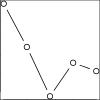
\includegraphics[width=0.45\textwidth]{jpg1.jpg}
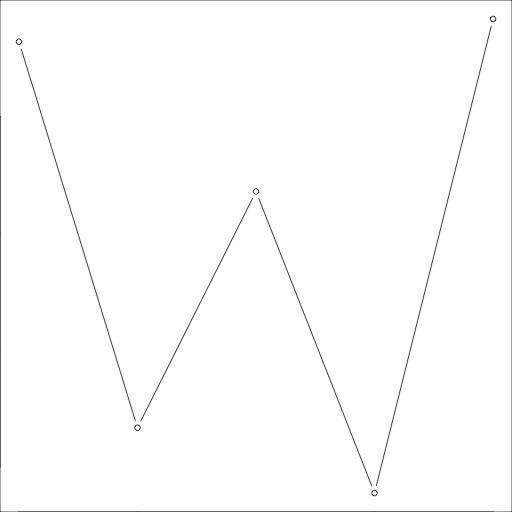
\includegraphics[width=0.45\textwidth]{jpg2.jpg}
\end{center}
Although the plot on the right hand side already has a higher quality, if you zoom in you will still notice that it contains some noise around the lines. Instead you could opt for a \texttt{png} image.
\begin{knitrout}
\definecolor{shadecolor}{rgb}{0.969, 0.969, 0.969}\color{fgcolor}\begin{kframe}
\begin{alltt}
\hlkwd{png}\hlstd{(}\hlstr{'png1.png'}\hlstd{,}\hlkwc{width}\hlstd{=}\hlnum{100}\hlstd{,}\hlkwc{height}\hlstd{=}\hlnum{100}\hlstd{)}
\hlkwd{par}\hlstd{(}\hlkwc{mar}\hlstd{=}\hlkwd{c}\hlstd{(}\hlnum{0}\hlstd{,}\hlnum{0}\hlstd{,}\hlnum{0}\hlstd{,}\hlnum{0}\hlstd{))}
\hlkwd{plot}\hlstd{(x,y,}\hlkwc{type}\hlstd{=}\hlstr{"b"}\hlstd{)}
\hlkwd{dev.off}\hlstd{()}

\hlkwd{png}\hlstd{(}\hlstr{'png2.png'}\hlstd{,}\hlkwc{width}\hlstd{=}\hlnum{512}\hlstd{,}\hlkwc{height}\hlstd{=}\hlnum{512}\hlstd{)}
\hlkwd{par}\hlstd{(}\hlkwc{mar}\hlstd{=}\hlkwd{c}\hlstd{(}\hlnum{0}\hlstd{,}\hlnum{0}\hlstd{,}\hlnum{0}\hlstd{,}\hlnum{0}\hlstd{))}
\hlkwd{plot}\hlstd{(x,y,}\hlkwc{type}\hlstd{=}\hlstr{"b"}\hlstd{)}
\hlkwd{dev.off}\hlstd{()}
\end{alltt}
\end{kframe}
\end{knitrout}
Compare the following two plots:
\begin{center}
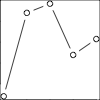
\includegraphics[width=0.45\textwidth]{png1.png}
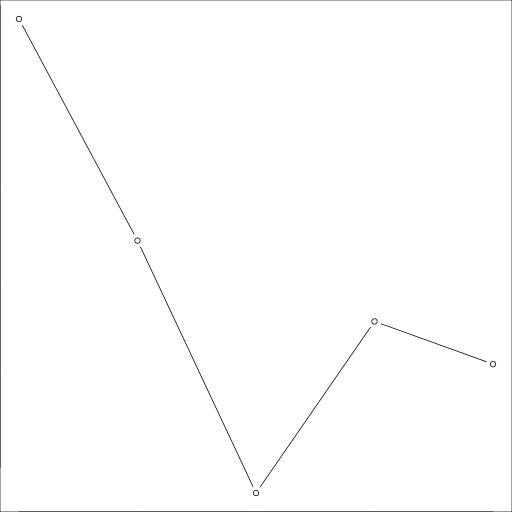
\includegraphics[width=0.45\textwidth]{png2.png}
\end{center}
Notice how the noise is now gone. The quality is however still not perfect. You can increase the quality by further increasing the \texttt{height} and \texttt{width} of the image. Alternatively you could also opt for a different file format: \texttt{pdf}: (Note that for this file format height and width can be specified but have a different meaning than for the previous file formats)
\begin{knitrout}
\definecolor{shadecolor}{rgb}{0.969, 0.969, 0.969}\color{fgcolor}\begin{kframe}
\begin{alltt}
\hlkwd{pdf}\hlstd{(}\hlstr{'pdf1.pdf'}\hlstd{)}
\hlkwd{par}\hlstd{(}\hlkwc{mar}\hlstd{=}\hlkwd{c}\hlstd{(}\hlnum{0}\hlstd{,}\hlnum{0}\hlstd{,}\hlnum{0}\hlstd{,}\hlnum{0}\hlstd{))}
\hlkwd{plot}\hlstd{(x,y,}\hlkwc{type}\hlstd{=}\hlstr{"b"}\hlstd{)}
\hlkwd{dev.off}\hlstd{()}
\end{alltt}
\end{kframe}
\end{knitrout}
\begin{center}
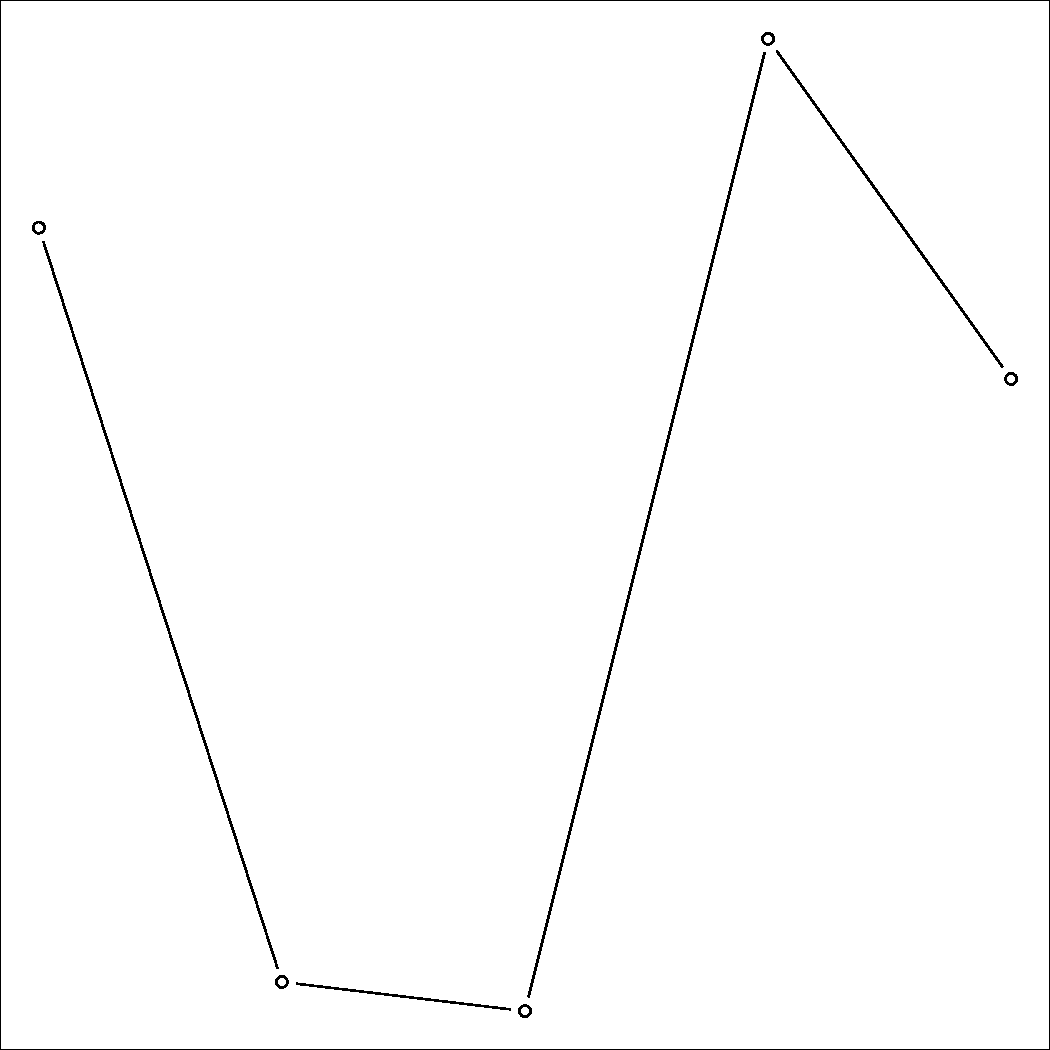
\includegraphics[width=0.45\textwidth]{pdf1.pdf}
\end{center}
Try to zoom in until you see the pixels: that's right, you can not find them. The \texttt{pdf} format is very high quality, but unfortunately this adventage is usually lost when you include it in a MS word document. You can however use them with full quality in \LaTeX documents. \LaTeX is also the program that we used for writing this pactical. If you want to try it without having to install anything and not even having to create an account:\\
\texttt{www.overleaf.com} \\
Some more file formats are available for creating pictures, for example \texttt{TIFF} and \texttt{BMP}. Realise how annoying it is if you made the perfect graph but saved it as a low quality file...
\end{mdframed}
\end{document}
